% Options for packages loaded elsewhere
\PassOptionsToPackage{unicode}{hyperref}
\PassOptionsToPackage{hyphens}{url}
%
\documentclass[
  11pt,
]{article}
\usepackage{amsmath,amssymb}
\usepackage{lmodern}
\usepackage{iftex}
\ifPDFTeX
  \usepackage[T1]{fontenc}
  \usepackage[utf8]{inputenc}
  \usepackage{textcomp} % provide euro and other symbols
\else % if luatex or xetex
  \usepackage{unicode-math}
  \defaultfontfeatures{Scale=MatchLowercase}
  \defaultfontfeatures[\rmfamily]{Ligatures=TeX,Scale=1}
  \setmainfont[]{Fira Sans Condensed}
  \setmonofont[]{Fira Code}
  \setmathfont[]{Fira Sans}
\fi
% Use upquote if available, for straight quotes in verbatim environments
\IfFileExists{upquote.sty}{\usepackage{upquote}}{}
\IfFileExists{microtype.sty}{% use microtype if available
  \usepackage[]{microtype}
  \UseMicrotypeSet[protrusion]{basicmath} % disable protrusion for tt fonts
}{}
\makeatletter
\@ifundefined{KOMAClassName}{% if non-KOMA class
  \IfFileExists{parskip.sty}{%
    \usepackage{parskip}
  }{% else
    \setlength{\parindent}{0pt}
    \setlength{\parskip}{6pt plus 2pt minus 1pt}}
}{% if KOMA class
  \KOMAoptions{parskip=half}}
\makeatother
\usepackage{xcolor}
\usepackage[margin=1in]{geometry}
\usepackage{graphicx}
\makeatletter
\def\maxwidth{\ifdim\Gin@nat@width>\linewidth\linewidth\else\Gin@nat@width\fi}
\def\maxheight{\ifdim\Gin@nat@height>\textheight\textheight\else\Gin@nat@height\fi}
\makeatother
% Scale images if necessary, so that they will not overflow the page
% margins by default, and it is still possible to overwrite the defaults
% using explicit options in \includegraphics[width, height, ...]{}
\setkeys{Gin}{width=\maxwidth,height=\maxheight,keepaspectratio}
% Set default figure placement to htbp
\makeatletter
\def\fps@figure{htbp}
\makeatother
\setlength{\emergencystretch}{3em} % prevent overfull lines
\providecommand{\tightlist}{%
  \setlength{\itemsep}{0pt}\setlength{\parskip}{0pt}}
\setcounter{secnumdepth}{-\maxdimen} % remove section numbering
\usepackage{amsmath}
\usepackage{multirow, multicol, booktabs}
\ifLuaTeX
  \usepackage{selnolig}  % disable illegal ligatures
\fi
\IfFileExists{bookmark.sty}{\usepackage{bookmark}}{\usepackage{hyperref}}
\IfFileExists{xurl.sty}{\usepackage{xurl}}{} % add URL line breaks if available
\urlstyle{same} % disable monospaced font for URLs
\hypersetup{
  pdftitle={Problem Set 6},
  pdfauthor={ECON 306 Fall 2022},
  hidelinks,
  pdfcreator={LaTeX via pandoc}}

\title{Problem Set 6}
\author{ECON 306 Fall 2022}
\date{\textbf{UNGRADED}: For Final Exam Practice Only}

\begin{document}
\maketitle

\hypertarget{concepts-and-critical-thinking}{%
\section{Concepts and Critical
Thinking}\label{concepts-and-critical-thinking}}

Please answer the following questions briefly (1-3 sentences). Use
examples as necessary. Be sure to label graphs fully, if appropriate.

\begin{enumerate}
\def\labelenumi{\arabic{enumi}.}
\tightlist
\item
  Compare and contrast the features of
\end{enumerate}

\begin{itemize}
\item
  \begin{enumerate}
  \def\labelenumi{\roman{enumi}.}
  \tightlist
  \item
    perfect competition
  \end{enumerate}
\item
  \begin{enumerate}
  \def\labelenumi{\roman{enumi}.}
  \setcounter{enumi}{1}
  \tightlist
  \item
    monopoly
  \end{enumerate}
\item
  \begin{enumerate}
  \def\labelenumi{\roman{enumi}.}
  \setcounter{enumi}{2}
  \tightlist
  \item
    oligopoly
  \end{enumerate}
\item
  \begin{enumerate}
  \def\labelenumi{\roman{enumi}.}
  \setcounter{enumi}{3}
  \tightlist
  \item
    monopolistic competition
  \end{enumerate}
\end{itemize}

Rank each of the above 4 market structures (from smallest/lowest to
largest/highest) in terms of:

\begin{itemize}
\item
  \begin{enumerate}
  \def\labelenumi{\roman{enumi}.}
  \tightlist
  \item
    the number of firms
  \end{enumerate}
\item
  \begin{enumerate}
  \def\labelenumi{\roman{enumi}.}
  \setcounter{enumi}{1}
  \tightlist
  \item
    long-run market price
  \end{enumerate}
\item
  \begin{enumerate}
  \def\labelenumi{\roman{enumi}.}
  \setcounter{enumi}{2}
  \tightlist
  \item
    equilibrium industry output
  \end{enumerate}
\item
  \begin{enumerate}
  \def\labelenumi{\roman{enumi}.}
  \setcounter{enumi}{3}
  \tightlist
  \item
    consumer surplus
  \end{enumerate}
\item
  \begin{enumerate}
  \def\labelenumi{\alph{enumi}.}
  \setcounter{enumi}{21}
  \tightlist
  \item
    long-run economic profits
  \end{enumerate}
\item
  \begin{enumerate}
  \def\labelenumi{\roman{enumi}.}
  \setcounter{enumi}{5}
  \tightlist
  \item
    deadweight loss
  \end{enumerate}
\end{itemize}

\clearpage

\begin{enumerate}
\def\labelenumi{\arabic{enumi}.}
\setcounter{enumi}{1}
\tightlist
\item
  Indicate based on the given information whether an industry is likely
  \textbf{perfectly competitive}, \textbf{monopolistically competitive},
  an \textbf{oligopoly}, or a \textbf{monopoly}:
\end{enumerate}

\begin{itemize}
\tightlist
\item
  Fairfax, Virginia has three movie theaters
\item
  Restaurants in the greater Piedmont area, with many different cuisines
  to choose from
\item
  All of Connecticut gets its electricity from Connecticut Light \&
  Power company
\item
  Laptops, where you can choose from many different brands (Acer, Asus,
  Gateway, Toshiba, Sony, HP, Dell, IBM, Lenovo, etc) and each is
  slightly different
\item
  Wheat in the U.S., provided by many small farmers, with each farmer's
  wheat being identical to every other farmer's wheat
\item
  The music industry, where Universal, Sony, EMI, and Warner account for
  87\% of the market \clearpage
\end{itemize}

\begin{enumerate}
\def\labelenumi{\arabic{enumi}.}
\setcounter{enumi}{2}
\tightlist
\item
  Indicate which good is more likely to have a \textbf{higher markup}
  for firms with market power in these industries, and why:
\end{enumerate}

\begin{itemize}
\tightlist
\item
  Alcohol or jewelry
\item
  Prescription drugs or televisions
\item
  Gym memberships or school supplies
\item
  Doughnuts or bread
\item
  Popcorn in a movie theater or popcorn from a street vendor
\end{itemize}

\vspace{3in}

\begin{enumerate}
\def\labelenumi{\arabic{enumi}.}
\setcounter{enumi}{3}
\tightlist
\item
  Describe the conditions required to make a market \emph{contestable.}
  Describe and compare the Nash equilibrium of a contestable market with
  a pure monopoly, and with perfect competition.
\end{enumerate}

\vspace{3in}

\begin{enumerate}
\def\labelenumi{\arabic{enumi}.}
\setcounter{enumi}{4}
\tightlist
\item
  Explain what a cartel is, and comment on their stability.
\end{enumerate}

\clearpage

\hypertarget{problems}{%
\section{Problems}\label{problems}}

Show all work for calculations. You may lose points, even if correct,
for missing work. Be sure to label graphs fully, if appropriate.

\begin{enumerate}
\def\labelenumi{\arabic{enumi}.}
\setcounter{enumi}{5}
\tightlist
\item
  Consider the following \emph{Entry game} in normal form. Suppose there
  are two firms, each of whom can choose to Enter a market, or Stay Out.
  If both firms enter, they split the market, each earning \$50. If both
  stay out, each firm earns \$0. If one enters and the other stays out,
  the entrant can act as a monopolist and earns \$100, with the other
  firm earning \$0.
\end{enumerate}

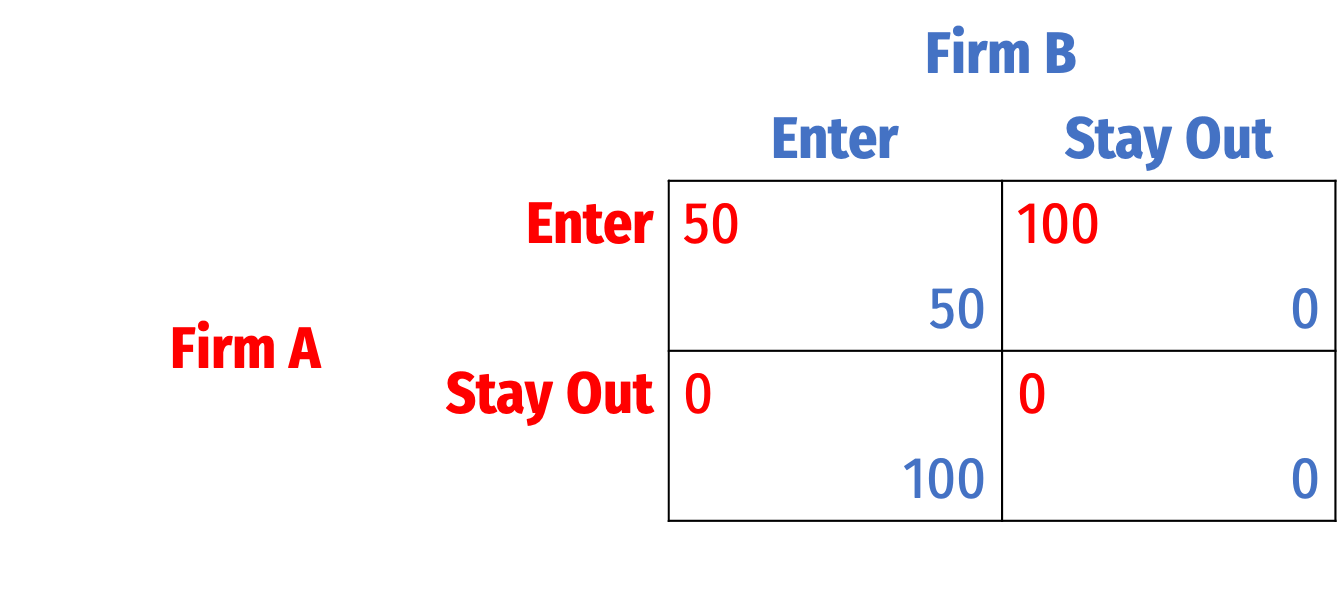
\includegraphics{../images/entrygame1.png}

What is the Nash Equilibrium of this game?

\clearpage

\begin{enumerate}
\def\labelenumi{\arabic{enumi}.}
\setcounter{enumi}{6}
\tightlist
\item
  Suppose you are a restaurant in a \textbf{monopolistically
  competitive} industry. Your firm has a constant marginal and average
  cost at \$4 per unit.
\end{enumerate}

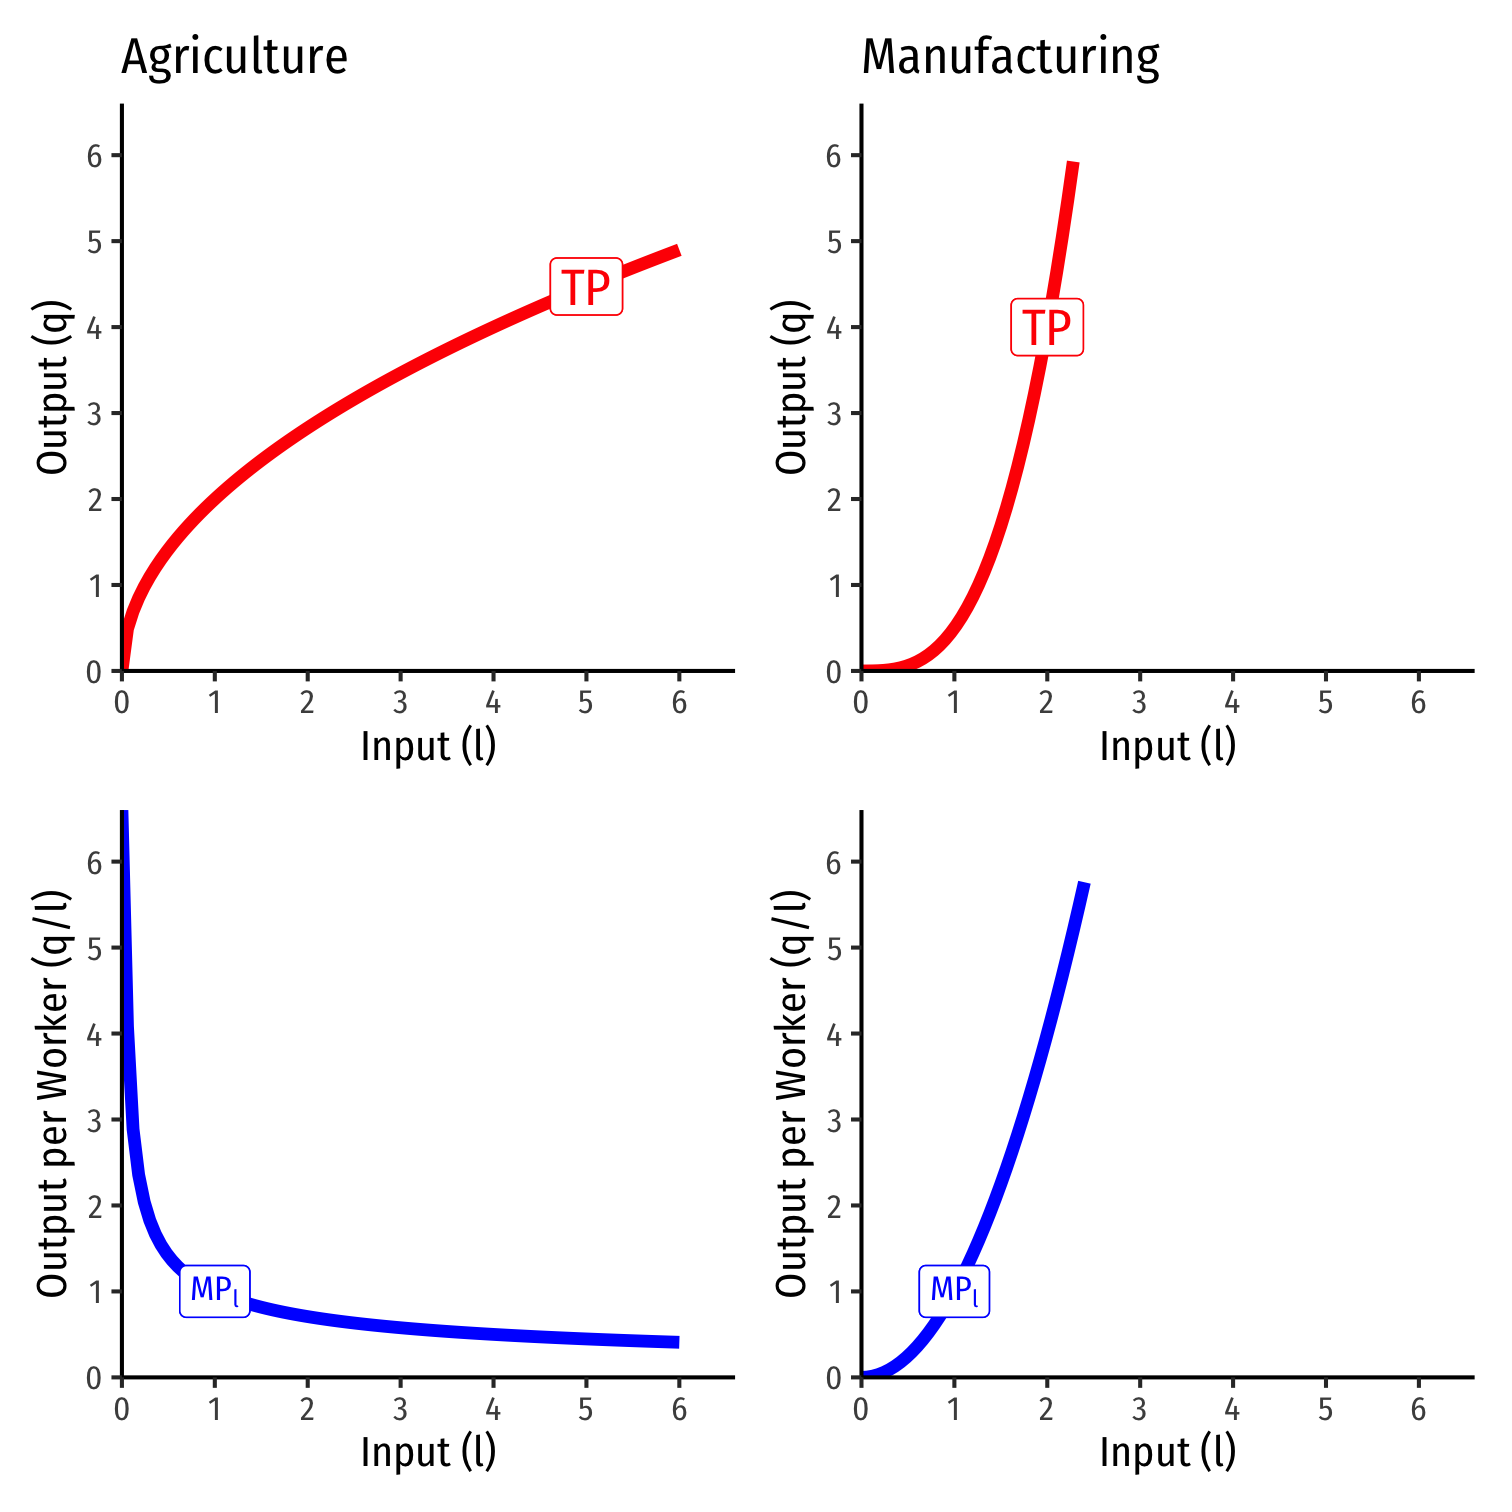
\includegraphics{06-problem-set-pdf_files/figure-latex/unnamed-chunk-1-1.pdf}

\begin{enumerate}
\def\labelenumi{\alph{enumi}.}
\tightlist
\item
  If this were a perfectly competitive market, what would be the market
  price and equilibrium quantity?
\item
  Calculate the (i) consumer surplus, (ii) profit, and (iii) deadweight
  loss at this price and quantity. Show these on the graph.
\item
  Now suppose this firm has market power from a barrier to entry, and
  can operate like a monopolist. What price and quantity does it set?
\item
  Calculate the (i) consumer surplus, (ii) profit, and (iii) deadweight
  loss at this price and quantity. Show these on the graph.
\item
  Now suppose that the firm had earned this market power via
  rent-seeking. From its lobbying efforts, it had convinced the local
  government to require all new restaurants to get a special license,
  making it harder for new entrants to compete in the market. What was
  the most that this firm was willing to spend on lobbying in order to
  get the license requirement?
\item
  If there are 10 identical (in terms of costs and size, if not food or
  brand) restaurants in the industry, and all engage in maximal
  rent-seeking to obtain the license, what is the true total cost of
  market power in this market to society?
\end{enumerate}

\clearpage

\begin{enumerate}
\def\labelenumi{\arabic{enumi}.}
\setcounter{enumi}{7}
\tightlist
\item
  You are a producer of smartphones and have some market power. You have
  a cost structure:
\end{enumerate}

\[\begin{aligned}
C(q)&=10q^2+200q+1000\\
MC(q)&=20q+200\\
\end{aligned}\]

You estimate the demand for your smartphones to be: \[q=100-0.2p\] where
\(q\) is millions of smartphones.

\begin{enumerate}
\def\labelenumi{\alph{enumi}.}
\tightlist
\item
  Find the function for your marginal revenues.
\item
  How many smartphones should you produce, and at what price, to
  maximize your profit?
\item
  What is the cost per smartphone at the quantity you are producing?
\item
  What is your total profit?
\item
  What would be the lowest possible price you would need to charge to
  break even?
\item
  How much of your price is markup over marginal cost?
\item
  Calculate the elasticity of demand at your profit-maximizing price.
\end{enumerate}

\clearpage

\begin{enumerate}
\def\labelenumi{\arabic{enumi}.}
\setcounter{enumi}{8}
\tightlist
\item
  Suppose that the market demand for bentonite is given by
  \[q = 40 - 0.5p\]
\end{enumerate}

where \(q\) tons of bentonite per day and \(p\) is the price per ton.
Bentonite is produced by a monopolist at a constant marginal and average
total cost of \$10 per ton.

\begin{enumerate}
\def\labelenumi{\alph{enumi}.}
\tightlist
\item
  Find the marginal revenue curve for the monopolist.
\item
  Find the profit-maximizing level of output and price.
\item
  How much profit does the monopolist earn?
\item
  How much of the price is markup over marginal cost?
\item
  Calculate the elasticity of demand at the profit-maximizing price.
\end{enumerate}

\clearpage

\begin{enumerate}
\def\labelenumi{\arabic{enumi}.}
\setcounter{enumi}{9}
\tightlist
\item
  \textbf{Optional: Section 1 (M/W) covered price discrimination in 4.3
  but we did not do any example problems. There will be no calculation
  problems requiring this on the final exam for either section.}
  Consider a boat rental firm on a popular beach that has a constant
  average and marginal cost of \$30 per boat hire. It has estimated that
  demand from Locals \((L)\) and demand from Tourists \((T)\) are:
  \[\begin{aligned}
  q_L&=40-0.4p\\
  q_T&=25-0.1p\\
  \end{aligned}\]
\end{enumerate}

\begin{enumerate}
\def\labelenumi{\alph{enumi}.}
\tightlist
\item
  Suppose it must charge a single price to all customers. Find the
  profit-maximizing quantity, price, and the total profits.
\item
  How much of the price is markup?
\item
  What is the price elasticity of demand at this price?
\item
  Now suppose the firm is able to segment the market and charge
  different prices to Tourists and Locals. Find the profit-maximizing
  quantity, price, and the total profits.
\item
  For each segment of the market: how much of the price is markup, and
  what is the price elasticity of demand at the optimal price? How did
  the price for each segment change from the single price (Part A), and
  why?
\end{enumerate}

\end{document}
